\chapter[Energia]{Energia}

Este capítulo apresentará a composição dos sistemas elétricos do projeto RICC e será dividido em três grandes seções referentes a cada um dos módulos do sistema.

A primeira abordará o dimensionamento do sistema fotovoltaico e dos componentes envolvidos na alimentação dos equipamentos eletrônicos da estação de medição. Assim, apresentados os cálculos, esquemáticos e simulações construídas para o projeto do sistema.

A segunda apresentará o dimensionamento do módulo atuador que será responsável por acionar remotamento o sistema de irrigação. Será dado enfoque no dimensionamento e simulações referentes a fonte de alimentação do sistema que foi projetada e será construída pelo próprio grupo.

Por fim, será apresentado o sistema de alimentação da central de comando. Vale ressaltar que o projeto da fonte foi realizado de modo a atender ambos os sistemas (Atuador e central) e de modo a ter sua saída regulada conforme a necessidade do sistema.

\section{Sistema Fotovoltaico \textit{Off-grid}}

Todo o embasamento teórico necessário para o dimensionamento de sistemas fotovoltaicos isolados foi apresentado no ponto de controle 1, assim como, um dimensionamento preliminar do sistema visando fornecer uma ideia inicial de custos.

Nesta etapa, será realizado o dimensionamento refinado do sistema apresentando todos os cálculos necessários, justificativa de escolha de componentes, alterações em relação ao primeiro dimensionamento e simulações computacionais validando os dados. 

O objetivo principal da análise atual é definir os diagramas elétricos e definir o processo de construção do subsistema de alimentação da estação de medição atentando se para a integração com os componentes eletrônicos e estruturais do projeto.

Todas as características climáticas necessárias para o dimensionamento do sistema fotovoltaico serão utilizadas levando em consideração que a estação encontra-se instalada no distrito federal. 

Neste trabalho serão usados os simbolos de fase e neutro para indicar respectivamente positivo e negativo nos diagramas unifilares apresentados. Além disso, todo cabeamento em vermelho será positivo e todo o cabeamento em preto será negativo. 

\subsection{Estruturação do sistema}

O sistema de alimentação fotovoltaico seguirá a seguinte estruturação:

\begin{figure}[H]
		\centering
		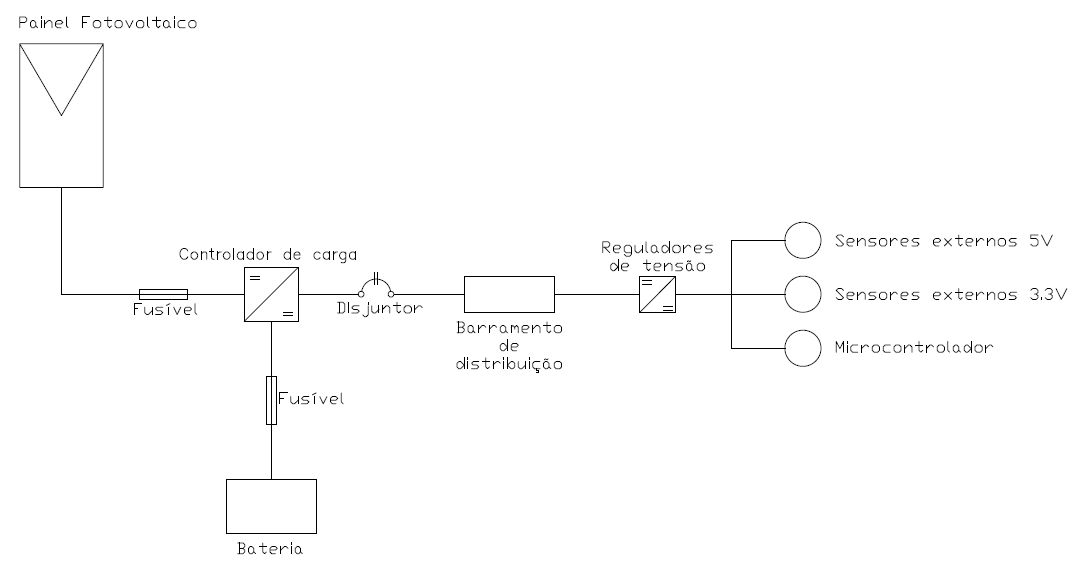
\includegraphics[width = .9 \textwidth]{energia/figuras/ene_pc2_01}
		\caption{Esquemático do sistema fotovoltaico. Fonte:Do Autor}
		\label{ene_pc2_01}
\end{figure}

A estruturação presente na figura \ref{ene_pc2_01} mostra um sistema \textit{Off-grid} genérico que será dimensionado e ajustado para se adequar as características do projeto. Assim, todo o capítulo consiste no dimensionamento de seus componentes de modo a finalizar o esquemático.

Para que o sistema atenda ao projeto, ele deve ser capaz de suprir a demanda de todos os componentes da estação, assim como, suprir as perdas de energia do sistema que serão encaradas como cargas adicionais neste trabalho. 

Deste modo, o dimensionamento do sistema teve início com o levantamento de carga da estação, que pode ser visto na tabela abaixo:

\begin{table}[H]
\centering
\caption{Levantamento de Cargas}
\resizebox{\textwidth}{!}{ 
\begin{tabular}{|c|c|c|c|c|c|c|}
\hline
\textbf{Componente} & \textbf{Quantidade} & \textbf{Corrente } & \textbf{Corrente total} & \textbf{Tensão } & \textbf{Consumo } & \textbf{Consumo diário } \\ 
& & \textbf{(A)} & &\textbf{(V)} & \textbf{(W)} & \textbf{(Wh/dia)} \\\hline
Sensor de umidadedo  & 3 & 0,005 & 0,015 & 5 & 0,075 & 1,8 \\ 
solo capacitivo & & & & & & \\\hline
Sensor de umidade e  & 1 & 0,00071 & 0,00071 & 3,3 & 0,002 & 0,056232 \\ 
temperatura do ar & & & & & & \\\hline
Sensor de temperatura  & 1 & 0,047 & 0,047 & 5 & 0,235 & 5,64 \\ 
do solo & & & & & & \\\hline
Sensor wattímetro & 1 & 0,005 & 0,005 & 3,3 & 0,017 & 0,396 \\ \hline
Pluviômetro & 1 & 0,05 & 0,05 & 3,3 & 0,165 & 3,96 \\ \hline
Anemômetro & 1 & 0,05 & 0,05 & 3,3 & 0,165 & 3,96 \\ \hline
Transceptor RF & 1 & 0,0126 & 0,0126 & 5 & 0,063 & 1,512 \\ \hline
Regulador de tensão & 4 & 0,005 & 0,02 & 5 & 0,100 & 2,4 \\ \hline
Led alta intensidade & 2 & 0,03 & 0,06 & 2,1 & 0,126 & 1,512 \\ \hline
Resistor led & 2 & 0,03 & 0,06 & 1,2 & 0,072 & 0,864 \\ \hline
Led difuso 3mm cores & 2 & 0,02 & 0,04 & 2,1 & 0,084 & 2,016 \\ \hline
Resistor led & 2 & 0,02 & 0,04 & 1,2 & 0,048 & 1,152 \\ \hline
Microcontrolador  & 1 & 0,24 & 0,24 & 3,3 & 0,792 & 19,008 \\ 
da estação & & & & & & \\\hline
 &  &  & 0,54031 & TOTAL & 1,944 & 44,28 \\ \hline
\end{tabular}
}
\label{ene_pc2_01_tab}
\end{table}

Para o cálculo do consumo diário de energia de cada sistema foi utilizada a seguinte equação:

\begin{equation}
E = P . t
\end{equation}

Sendo E a energia demandada diariamente pelo componente, P sua potência de trabalho e t o número de horas de funcionamento diárias.

Foi considerado a potência nominal média indicada no datasheet do componenete para realização dos cálculos. Além disso, considerou-se o tempo de funcionamento de 24 h por dia para os sensores com excessão dos leds de alta intensidade que serão acionados apenas durante a noite (12 h por dia).  

De posse do consumo diário de energia, passou se para estimativa das perdas no sistema de modo a permitir o dimensionamento dos componentes.

\subsection{Perdas do sistema}

Para o dimensionamento do sistema todas as perdas de energia serão consideradas como cargas que precisam ser supridas pelo sistema fotovoltaico. O esquemático abaixo apresenta as perdas consideradas.

\begin{figure}[H]
		\centering
		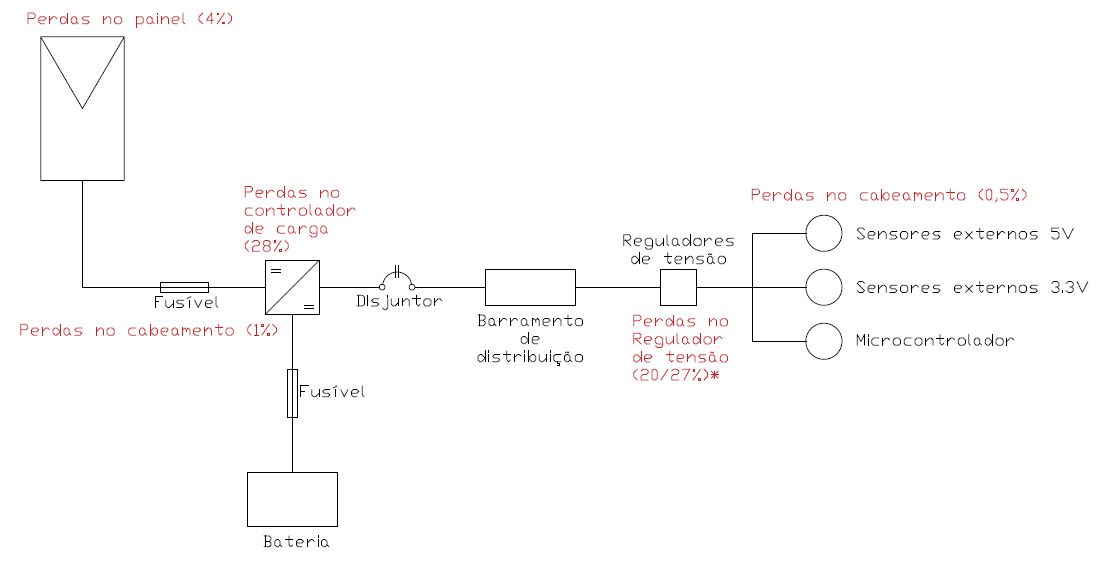
\includegraphics[width = .9 \textwidth]{energia/figuras/ene_pc2_02}
		\caption{Esquemático de perdas de sistema fotovoltaico. Fonte:Do Autor}
		\label{ene_pc2_02}
\end{figure}

O esquemático apresenta as principais perdas do sistema em relação a seus componentes, para melhor explicação dos valores adotados será apresentado uma breve explicação de cada um e a metodologia de definição dos valores de cada um.

\subsubsection{Perdas no painel}

As principais perdas de energia referentes aos painéis fotovoltaicos são provenientes da orientação do módulo, sombreamento, acúmulo de sujeira e mismatch.
 
Como o projeto contará apenas com uma placa fotovoltaica, não haverá perdas por mismatch já que estas estão relacionadas ao descasamento de dois ou mais módulos. Além disso, não haverá perdas por sombreamento, pois o equipamento será instalado em campo aberto e será mais alto que a cultura em questão. Por fim, será indicado no procedimento de montagem da estação que o painel deve ficar direcionado para o norte e com a inclinação condizente com a latitude segundo a tabela \ref{ene_pc2_02_tab}, de modo que não serão consideradas perdas provenientes da orientação do painel.

\begin{table} [H]
\centering
\caption{Angulação dos painéis. \cite{Villalva}}
\begin{tabular}{|c|c|}
\hline
\textbf{Latitude geográfica do local} & \textbf{ângulo de inclinação recomendado}\\
\hline
$0\,^{\circ}\mathrm{C}$ a $10\,^{\circ}\mathrm{C}$& $10\,^{\circ}\mathrm{C}$ \\
\hline
$11\,^{\circ}\mathrm{C}$ a $20\,^{\circ}\mathrm{C}$&  latitude\\
\hline
$21\,^{\circ}\mathrm{C}$ a $30\,^{\circ}\mathrm{C}$& latitude + $5\,^{\circ}\mathrm{C}$\\
\hline
$31\,^{\circ}\mathrm{C}$ a $40\,^{\circ}\mathrm{C}$ &  latitude + $10\,^{\circ}\mathrm{C}$\\
\hline
mais de $40\,^{\circ}\mathrm{C}$ &  latitude + $15\,^{\circ}\mathrm{C}$ \\
\hline
\end{tabular}
\label{ene_pc2_02_tab}
\end{table}	
 
	Desta forma a única perda considerada no painel será proveniente do acúmulo de poeira ou outros dejetos. Está perda pode chegar a 15\% da energia produzida em locais secos, sendo a limpeza periódica indispensável. Em termos médios, o acúmulo de poeira provoca perdas de 4\% ao ano. \cite{zorrilla}. 
	
	Como as condições específicas de operação da estação não são definidas já que ela pode atuar em diversas plantações, será assumido o valor médio de 4\% de perdas devido a acúmulo de poeira. Além disso, será indicado no manual de manutenção que os painéis devem ser limpos para manter a eficiência do sistema.

\subsubsection{Perdas no controlador de carga} 

	Como definido no relatório anterior, será utilizado um controlador de carga de PWM para realizar o controle da bateria. Este controlador transmite a energia proveniente dos painéis para a bateria através de pulsos cíclicos que podem atingir frequências de centenas de ciclos por segundo. Desta forma, ela consegue manter a tensão das baterias em um nível mais constante e reduzir o tempo que os painéis permanecem desacoplados da bateria, consequentemente aumentando a eficiência do sistema. \cite{SAAD}.
	
	Porém, sua eficiência é limitada pela tensão de operação da bateria. Por exemplo, considere um painel fotovoltaico de 90 Wp com tensão nominal de 17,06 V e corrente nominal de 5,28 A (referência do painel sinosola SA90-64P). Caso seja utilizado um controlador de carga PWM de 12,5 V (Tensão de saída para bateria) a potência transmitida será de 12,5V * 5,28 totalizando 66 W, ou seja, apenas 73,3\% da potência será transmitida para a bateria.
	
	O valor das perdas no controlador de carga foi calculado utilizando o mesmo método apresentado acima com os valores de referência do modelo de painel e do controlador escolhido e com todos os cálculos detalhados na seção de dimensionamento do controlador. 
	
	Como os controladores PWM apresentam eficiências que variam de 70 a 75 \% em média foi utilizado um valor inicial de 70 \% de rendimento de modo a calcular a potência dos módulos fotovoltaicos, escolher um modelo e depois dimensionar o controlador para ele de modo a obter a eficiência real do controlador para está situação. Em seguida, foi realizado mais uma interação aplicando a real eficiência do controlador e analisando se o painel ainda era o mais indicado para a situação.

\subsubsection{Perdas no regulador de Tensão}

	O regulador de tensão é um dispositivo que realiza a conversão DC/DC da tensão disponibilizada pela bateria para a tensão de operação dos sensores e componentes eletrônicos. No projeto, será utilizado o módulo regulador de tensão LM2596, este módulo consegue trabalhar em uma ampla faixa de tensões de entrada e ser regulado para uma tensão específica de saída. 
	
	Este módulo é um conversor CC-CC Buck com dispositivo de comutação semi-condutor chaveado, o que aumenta sua eficiência em relação aos modelos de regulador lineares. Assim, o componente foi escolhido levando em conta sua maior eficiência, custo de aquisição e padronização do sistema, pois como ele pode ser regulado para obter uma saída expecífica a partir da entrada de 12V da bateria, pode-se utilizá-lo em todos os pontos de regulação da estação.	
	
	A porcentagem de perdas foi definida de acordo com o datasheet do componente e suas curvas de eficiência. Quanto maior a diferença entre a tensão de entrada e a tensão de saída do regulador, menor será a eficiência da conversão. Por isso, são apresentados dois valores de perdas no regulador sendo o de 20\% para a regulação de 12V para 5V e o de 27\% para a regulação de 3.3 V. Tais regulações e expecíficações serão abordadas mais profundamente no decorrer do capítulo.
	
\subsubsection{Perdas no cabeamento}

	Todos os sistemas de cabeamento foram dimensionados de modo a se manterem dentro do limite máximo de queda de tensão estipulado de 1,5\%.
	
	Esse limite será subdividido em duas partes para os circuitos de alimentação e circuitos de distribuição. Essa divisão foi considerada apenas para o cálculo da queda de tensão nos trechos do circuito e não existe fisicamente.
	 
	Será considerado circuito de alimentação o cabeamento que conecta a placa fotovoltaica ao quadro e o cabeamento que conecta a bateria ao quadro. Estes cabeamentos foram projetados de modo a apresentarem perdas de até 1\%.
	
	Por fim, será considerado circuito de distribuição todo o cabeamento que parte do quadro e visa alimentar os sensores e demais componentes da estação. Este circuito também foi dimensionado de modo a apresentar perdas de até 0,5\%.

\subsection{Dimensionamento do Painel Solar}

Os painéis fotovoltaicos são as estruturas responsáveis por gerar a energia que abastecerá todos os componentes da estação de medição. Deste modo, eles são dimensionados para atender a demanda de energia diária mais as perdas inerentes ao sistema.

\begin{equation}
	E_C = \sum(C.t) + Perdas
\end{equation}

	Sendo $E_c$ a energia consumida diariamente, C a potência do equipamento e t o tempo de uso. As perdas são dadas pela equação:
	
\begin{equation}
	Perdas = \sum (C . t . \eta)
\end{equation}	
	
	Com $\eta$ sendo a porcentagem de perdas a qual a energia está exposta.
	
	Como apresentado no início do capítulo o consumo de energia dos equipamentos eletrônicos é de 44,28 $Wh/dia$ e as perdas totais do sistema variam entre 53 a 60\%. Assim, a energia consumida diariamente é de:

\begin{equation}
E_C = 44,28 + (11,35 . 0,53) + (32,93 . 0,6) = 70.05 \dfrac{Wh}{dia}
\label{consumo}
\end{equation}

	Na equação \ref{consumo} a primeira parcela de perdas se refere aos componentes alimentados em 5v e a segunda aos componentes alimentados em 3,3v.

	Em seguida é necessário obter os dados de potência solar para efetuar o cálculo da potência do painel. Como foi definido que o estudo de caso será realizada considerando uma plantação no distrito federal foram obtidos os dados de irradiação mensal deste local através do CRESESB. 
	
\begin{table}[H]
\centering
\caption{Irradiação solar média em Brasília. \cite{crecesb}}
\resizebox{\textwidth}{!}{%
\begin{tabular}{|c|c|c|c|c|c|c|c|c|c|c|c|c|c|c|}
\hline
\multirow{2}{*}{\textbf{Ângulo}} & \multirow{2}{*}{\textbf{Inclinação}} & \multicolumn{13}{c|}{\textbf{Irradiação solar diária média mensal (kWh/$m^2$ dia)}} \\ \cline{3-15} 
 &  & \multicolumn{1}{l|}{Jan} & \multicolumn{1}{l|}{Fev} & \multicolumn{1}{l|}{Mar} & \multicolumn{1}{l|}{Abr} & \multicolumn{1}{l|}{Mai} & \multicolumn{1}{l|}{Jun} & \multicolumn{1}{l|}{Jul} & \multicolumn{1}{l|}{Ago} & \multicolumn{1}{l|}{Set} & \multicolumn{1}{l|}{Out} & \multicolumn{1}{l|}{Nov} & \multicolumn{1}{l|}{Dez} & \multicolumn{1}{l|}{Média} \\ \hline
Plano horizontal & 0$\,^{\circ}\mathrm{C}$ N & 5,42 & 5,74 & 5,05 & 5,06 & 4,83 & 4,7 & 4,95 & 5,77 & 5,7 & 5,59 & 5,08 & 5,44 & 5,28 \\ \hline
Ângulo de latitude & 16 $\,^{\circ}\mathrm{C}$ N & 5,01 & 5,5 & 5,1 & 5,46 & 5,56 & 5,61 & 5,83 & 6,47 & 5,91 & 5,45 & 4,75 & 4,98 & 5,47 \\ \hline
\end{tabular}%
}
\label{ene_pc2_03_tab}
\end{table}

A partir dos dados de irradiação é possível calcular as horas de sol pleno diárias através da equação:

\begin{equation}
HSP = \dfrac{I}{1 \dfrac{kW}{m^2}}
\end{equation}

Sendo HSP o número de horas de sol pleno e I a irradiação solar. Para sistemas isolados, deve-se escolher o menor valor de irradiação proveniente da tabela no ângulo de interesse e assegurando que o sistema conseguirá abastecer a carga mesmo no mês com menor incidência solar. No caso do trabalho, esse valor será igual a 4,75 kWh/m² dia.

	De posse destas informações é possível calcular a potência de pico do sistema.
	
\begin{equation}
P_p = \dfrac{E_c}{HSP} = 14,748 W_p
\end{equation}

	Como não há modelo comercial de placa fotovoltaica nesta medida, foi escolhido utilizar o modelo comercial imediatamente superior de 20 Wp. Por fim, optou-se pelo painel fotovoltaico da marca Yingli modelo YL020P-17b. \cite{yingli}

	A energia gerada por um módulo fotovoltaico varia de acordo com sua temperatura de operação, pois conforme exposto no primeiro ponto de controle o aumento da temperatura do módulo promove a diminuição da tensão de saída da placa consequentemente reduz a potência gerada.
	
	Para calcular a redução da potência do painel devido a temperatura é necessário conhecer as variáveis da placa e a temperatura média a qual ele trabalhará. Assim, a tabela \ref{ene_pc2_04_tab} apresenta a variação das grandezas do módulo segundo a temperatura e a tabela \ref{ene_pc2_05_tab} apresenta a temperatura média para o distrito federal. 
	
\begin{table}[H]
\centering
\caption{Coeficientes de variação térmica da placa solar}
{%
\begin{tabular}{|l|c|}
\hline
\multicolumn{1}{|c|}{\textbf{Grandezas}} & \textbf{Coeficientes de variação} \\ \hline
Coeficiente de Temperatura da Potência(Pm) & -0,45 \%/$\,^{\circ}\mathrm{C}$ \\ \hline
Coeficiente de Temperatura da Corrente(Isc) & 0,06 A/$\,^{\circ}\mathrm{C}$ \\ \hline
Coeficiente de Temperatura da Voltagem(Voc) & -0,37 V/$\,^{\circ}\mathrm{C}$ \\ \hline
\end{tabular}%
}
\label{ene_pc2_04_tab}
\end{table}

\begin{table}[H]
\centering
\caption{Temperatura média mensal. \cite{climate}}
\resizebox{\textwidth}{!}{%
\begin{tabular}{|c|c|c|c|c|c|c|c|c|c|c|c|c|}
\hline
\textbf{} & \textbf{Jan} & \textbf{Fev} & \textbf{Mar} & \textbf{Abr} & \textbf{Mai} & \textbf{Jun} & \textbf{Jul} & \textbf{Ago} & \textbf{Set} & \textbf{Out} & \textbf{Nov} & \textbf{Dez} \\ \hline
Temperatura média ($\,^{\circ}\mathrm{C}$) & 21.9 & 21.9 & 21.7 & 20.8 & 19.6 & 18.9 & 19.9 & 21.3 & 22.3 & 22.1 & 21.7 & 21.3 \\ \hline
Temperatura mínima ($\,^{\circ}\mathrm{C}$) & 17.1 & 17 & 16.7 & 15.3 & 13.5 & 12.5 & 13.3 & 14.8 & 16.7 & 17.2 & 17.1 & 16.1 \\ \hline
Temperatura máxima ($\,^{\circ}\mathrm{C}$) & 26.7 & 26.9 & 26.7 & 26.3 & 25.7 & 25.3 & 26.5 & 27.9 & 27.9 & 27 & 26.3 & 26.5 \\ \hline
\end{tabular}%
}
\label{ene_pc2_05_tab}
\end{table}

A como no caso da irradiação, deve-se utilizar o mês com maior temperatura máxima de modo a garantir que o sistema consiga suprir a carga durante todos os períodos do ano. Assim, será utilizado o valor de $27,9\,^{\circ}\mathrm{C}$ como temperatura máxima.

A temperatura média da célula fotovoltaica em operação vai ser sempre superior à temperatura ambiente devido ao efeito fotovoltaico e as perdas Ôhmicas. De modo geral, pode-se calcular a temperatura do módulo através da seguinte equação:

\begin{equation}
T_{mod} = T_{amb} + kt . G
\end{equation}

	Sendo $T_{mod}$ a temperatura na superfície do módulo, $T_{amb}$ a temperatura ambiente, kt a constante térmica para o módulo que pode ser adotada como $0,03\,^{\circ}\mathrm{C}$ e G é a irradiância média de teste sobre o módulo que pode ser adotada como 1000 $W/m^2$. 
	
	Assim a temperatura do módulo é:

\begin{equation}
T_{mod} = 27,9 + (0,03 . 1000) = 57,9 \,^{\circ}\mathrm{C}
\end{equation}

Com a temperatura de operação do módulo é possível descobrir a queda da potência produzida em relação a temperatura de testes utilizando os coeficientes de variação apresentados.

\begin{equation}
P_{real} =P . (1 + C_p . (T_{mod} - T_{test}))
\end{equation}


	Sendo $P_{real}$ a potência real gerada pelo módulo, P a potência de teste que para o modelo escolhido é de 20 W, $C_p$  é o coeficiente de variação da potência em função da temperatura e $T_{test}$ é a temperatura de teste do módulo que é adotada como $25\,^{\circ}\mathrm{C}$.
	
	Assim, a potência real gerada pelo módulo é de:

\begin{equation}
Preal= 20 . (1 + (- 0,45/100) . (57,9 - 25)) = 17,04 W
\end{equation}

Deste modo, é possível concluir que o painel fotovoltaico apresentará uma potência maior do que a potência consumida, mesmo no mês com maiores temperaturas no ano, assegurando o suprimento de energia para a estação. 

Por fim, é possível utilizar os dados de irradiação mensal e de temperatura média para determinar a geração de energia do sistema. A figura \ref{ene_pc2_02} apresenta a relação entre geração e consumo no decorrer do ano.

\begin{figure}[H]
		\centering
		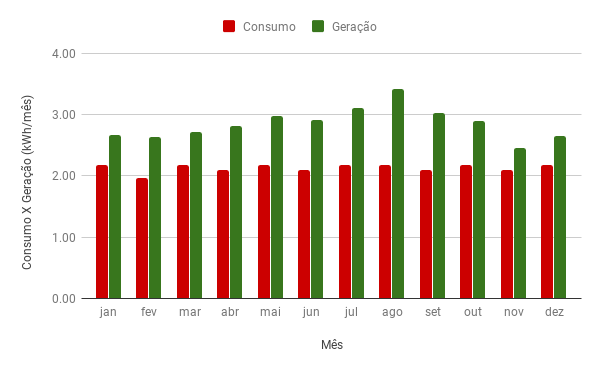
\includegraphics[width = .9 \textwidth]{energia/figuras/ene_pc2_03}
		\caption{Geração x Consumo. Fonte:Do Autor}
		\label{ene_pc2_03}
\end{figure}

É possível observar que a energia produzida pelo sistema fotovoltaico é superior a energia consumida em todos os meses do ano. Esse fato ocorre porque o modelo comercial de 20W é maior do que o necessário para a alimentação do sistema. Contudo, o modelo diretamente inferior de 10 W não consegue suprir a demanda energética de modo que é necessário usar o modelo previsto.

	Vale ressaltar que a energia adicional permitirá que as baterias sejam carregadas mais rapidamente e tornará o sistema mais robusto já que conseguirá absorver perdas maiores de energia sem comprometer a alimentação das cargas.

\subsection{Dimensionamento da Bateria}


	O sistema de baterias será responsável por armazenar a energia excedente produzida durante o dia para ser utilizada em momentos de pouca ou nenhuma geração. Para dimensionar a bateria necessária ao projeto é utilizada a seguinte equação:

\begin{equation}
Bat_{c20} = \dfrac{(C_c + Perdas). N}{\eta . V}  
\end{equation}

	Sendo $Bat_{c20}$ a capacidade da bateria em Ah, $C_c$ o consumo diário dos equipamentos da estação, N o número de dias de autonomia, $\eta$ a profundidade de descarga da bateria e V a tensão da bateria.
	
	As perdas apresentadas no dimensionamento da bateria não são as mesmas utilizadas no dimensionamento dos painéis, já que as perdas por acúmulo de sujeira e eficiência do controlador de carga não se aplicam. Desta forma, a bateria enxerga apenas cerca de 21 a 28\% de perdas que são provenientes da eficiência do regulador e das perdas nos cabos.
	
	Como requisito de projeto, foi definido que o sistema apresentará autonomia de três dias. Além disso, para o projeto de PI2, foi decidido que será usado 100\% de capacidade de descarga já que se trata de um protótipo apenas e não é necessário que ele tenha uma vida útil muito longa. Por fim, será utilizado baterias de 12 V, pois estas são mais fáceis de comprar e em geral mais baratas que as de tensões superiores.
	
Assim, a capacidade da bateria para o projeto será de:

\begin{equation}
Batc20 = \dfrac{(44,28 + (11,35 . 0,21) + (32,93 . 0,28)) . 3}{12} = 13,97 Ah 
\end{equation}

	A capacidade encontrada é difícil de ser encontrada em modelos comerciais de modo que serão utilizadas duas baterias de 7 Ah conectadas em paralelo. A conexão em paralelo permite que ambas as baterias colaborem enviando corrente ao circuito e dessa forma criando uma capacidade conjunta de 14 Ah que é aproximadamente o valor necessário.
	
	Segundo o manual das baterias da Unipower, quando é utilizado uma profundidade de descarga de 100\% a vida útil da bateria é de cerca de 200 ciclos. Para o caso de aplicação real do produto seria aplicado uma profundidade de descarga de 50\% aumentando a vida útil para mais de 600 ciclos. \cite{unipower}
	
	Esta consideração foi informada a estrutura de modo que a estação consiga comportar a nova bateria (Bateria do caso comercial) sem precisar de nenhuma mudança estrutural. 
	
	A bateria escolhida para ser usada no projeto será a bateria estacionária selada VRLA 12V 7Ah UP1270SE da Unipower. As baterias serão ligadas através do esquemático \ref{ene_pc2_04}.
	
\begin{figure}[H]
		\centering
		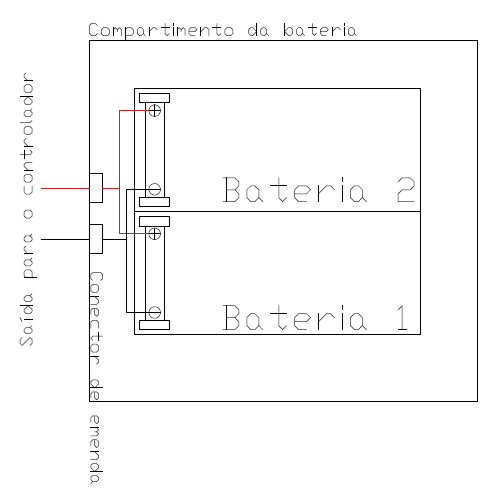
\includegraphics[width = .9 \textwidth]{energia/figuras/ene_pc2_04}
		\caption{Conexão do banco de barias. Fonte:Do Autor}
		\label{ene_pc2_04}
\end{figure}

	Serão utilizados conectores de emenda para fios de modo a realizar a conexão das duas baterias em paralelo com o controlador de carga. Esse tipo de conector substitui a conexão manual dos cabos sendo mais confiável e reduzindo a resistência de contato de modo a reduzir as perdas no cabeamento.
	
	Além disso, serão usados terminais de luva fêmea para realizar a conexão entre os fios e os terminais da bateria.

\subsection{Dimensionamento do Controlador de carga}

	Para o dimensionamento de um controlador de carga deve-se levar em conta a potência gerada pelos painéis fotovoltaicos e a tensão de operação do sistema de bateria. Assim, é possível calcular a corrente de trabalho do componente e escolher o modelo que melhor atenda a necessidade do projeto.
	
	Dessa forma, temos:

\begin{equation}
C_o = \dfrac{P_g}{V} = \dfrac{20}{16,6} = 1,2 A
\end{equation}

	Sendo $C_o$ a corrente de operação, $P_g$ a potência gerada pelos painéis e V a tensão dos painéis. Além disso, deve-se calcular a corrente demandada pela carga e a corrente de curto circuito do painel de modo a assegurar que o controlados aguente todas as correntes que possa ser exposto.
	
	No caso do projeto, os sensores e componentes elétricos demandam uma corrente total de 0,4552 A. Além disso, o manual do painel aponta que sua corrente nominal de operação é de 1,2 A e sua corrente de curto circuito é de 1,31 A de modo que o controlador deve suportar a máxima corrente que pode passar por ele (1,31 A).
	
	Comercialmente o modelo de controlador de carga com menor corrente de operação apresenta corrente de 5 A o que é suficiente para o projeto e permitirá um sistema robusto e com menos probabilidade de queima do controlador.
	
	O controlador de carga escolhido para aplicação foi o modelo Epsolar Landstar LS0512E 5A 12V. Ele apresenta a tecnologia PWM e atende os critérios expostos no ponto de controle 1, além disso, é compatível com a placa e com a bateria escolhida, apresenta rapidez na entrega e custos compatíveis com o orçamento do projeto.
	
	Por fim, a eficiência deste controlador é calculada utilizando as características do painel escolhido. A placa apresenta tensão nominal de 16,6 V e corrente nominal de 1.2 A o que totaliza sua potência nominal de 20 W, como o controlador PWM reduz a tensão enviada pelo painel de modo a carregar a bateria, temos que a potência entregue pelo controlador é de 14.4 W, ou seja, apenas 72 \% da potência de pico do painel. 


\subsection{Dimensionamento do Quadro de Proteção}

O quadro de proteção da estação seguirá o seguinte esquemático:

\begin{figure}[H]
		\centering
		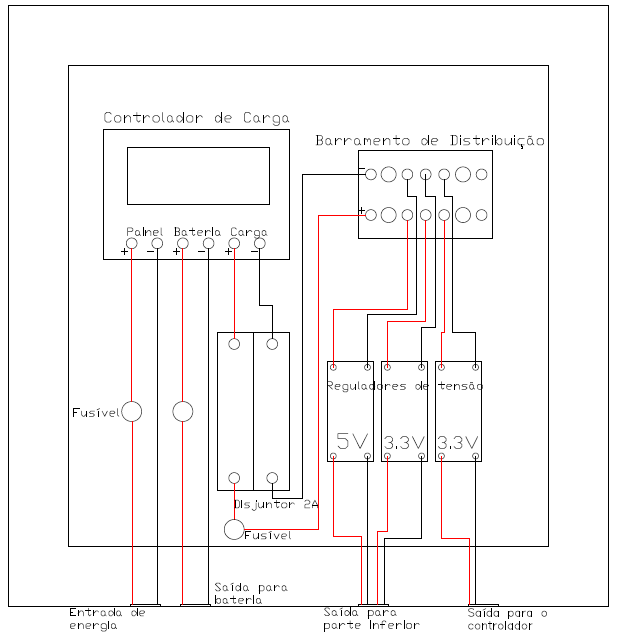
\includegraphics[width = .9 \textwidth]{energia/figuras/ene_pc2_05}
		\caption{Esquemático do quadro de proteção. Fonte:Do Autor}
		\label{ene_pc2_05}
\end{figure}

O quadro foi projetado de modo a proteger o controlador de carga, deste modo há um fusível entre os painéis solares e o controlador e um entre a bateria e o controlador. Além disso, haverá um disjuntor entre o controlador de carga e o barramento de distribuição para proteger os dispositivos eletrônicos e servir de chave de secção para deserneginar os componentes e permitir sua manutenção em segurança.

Para o dimensionamento dos dispositivos de proteção foi levado em consideração a corrente máxima que poderá fluir por cada circuito e a corrente máxima do controlador de modo a garantir sua proteção. Ainda, utilizou-se um coeficiente de segurança de 25 \% sobre o valor máximo de corrente conforme exposto como parâmetro de segurança no ponto de controle 1.

A corrente máxima que pode fluir no circuito entre a placa fotovoltaica e o controlador é de 1,31 A, utilizando o fator de segurança e adotando o componente comercial mais próximo do resultado obtido foi adotado um fusível de 2A. Este fusível estará conectado ao circuito através de um porta fusível 5x20 AS-06 de modo a garantir melhor conexão e facilitar a substituição do fusível em caso de falha.

Para o circuito entre a bateria e o controlador também foi adotado um fusível de 2A conectado ao circuito através de um porta fusível de 5x20 AS-60. Esse valor foi escolhido de modo a padronizar os fusíveis de proteção e evitar erros futuros de utilização, além de evitar que a corrente que passe pelo controlador de carga seja muito alta e venha causar danos. Dos componentes do sistema, as baterias são as únicas capazes de gerar correntes altas o suficiente para queimar o controlador de carga, assim, ao utilizar esse fusível em um nível de corrente mais baixa garantiremos a proteção do controlador.

Para proteção dos componentes eletrônicos será usado uma combinação de disjuntor em série com fusível. Está estrutura serão usada, pois a corrente total que flui para os sensores é muito baixa para um disjuntor conseguir atuar como dispositivo de proteção. Assim, o disjuntor funcionará como uma chave de seccionamento desenergizando os componentes e permitindo sua manutenção segura enquanto que o fusível funcionará como dispositivo de proteção evitando que sobrecorrentes queimem os componentes. 

Para a escolha destes componentes, foi considerada a corrente total dos componentes eletrônicos de 0,54 A, assim como, um coeficiente de segurança de 1,25. Deste modo o modelo comercial de fusível que melhor atende a aplicação é um fusível de 0,7 A. Em seguida, pesquisou-se modelos de disjuntores para serem usados e optou-se pela utilização de um disjuntor bipolar de 2 A curva C.

Foi escolhido utilizar um disjuntor no lugar da chave seccionadora pela disponibilidade do componente e por seu custo. Durante as pesquisas realizadas, foi difícil encontrar chaves seccionadoras de 2 A, sendo estas projetas para correntes maiores e consequentemente tendo um maior custo que o disjuntor escolhido (o valor médio da chave encontrada foi cerca de duas vezes mais alto que o do diajuntor). Por fim, o disjuntor apresenta a vantagem de evitar a formação de arcos elêtricos durante sua abertura o que é mais uma vantagem em sua utilização.

Após os dispositivos de proteção, o controlador de carga se liga ao quadro de distribuição energizando 6 barramentos distintos que podem ser utilizados para alimentar as cargas. No caso do projeto, apenas quatro deles serão utilizados, sendo os demais deixados em \textit{stand-by} e dispooníveis para mudanças futuras no projeto.

O controlador de carga fornece energia em cerca 12 V, que é a tensão nominal da bateria, porém os componentes eletrônicos não podem ser alimentados neste nível de tensão. Desta forma, há um estágio de reguladores de tensão na saída do barramento de distribuição visando abaixar o nivel de tensão e permitir a alimentação das cargas.

Os reguladores escolhidos para o projeto serão módulos reguladores buck LM2596 com dispositivos semi-condutores chaveados. Estes módulos apresentam eficiências de conversão superiores aos antigos modelos lineares, além de serem mais robustos e aceitarem uma ampla gama de tensões de entrada produzindo saídas específicas de acordo com a definição de seu \textit{duty-cycle}.

Ainda, foi consultado o datasheet do módulo de modo a obter as curvas de eficiência de conversão de energia e a partir delas foi encontrado a porcentagem de perdas expostas na seção de perdas no sistema.

As cargas foram subdivididas em três subconjuntos de acordo com seu posicionamento físico na estrutura e com seu nível de tensão. Sendo assim, foram divididas em componentes superiores, inferiores e centrais  de modo que escolheu-se usar três reguladores de tensão sendo um para cada subgrupo. Este arranjo aumenta a robustez do sistema, pois se um regulador parar de funcionar os demais continuarão e reduz a perda de energia em conexões e derivações por tornar os circuitos mais específicos e diretos.

Por fim, todos os componentes ficarão localizados dentro de um quadro de comando IP65 localizado na estrutura. Este quadro permitirá a proteção dos componentes de intemperies e sua organização já que conta com uma placa de montagem para fixação dos componentes e ordenação da fiação. Este mesmo quadro será utilizado como estrutura para o atuador apresentado posteriormente.

Os componentes serão presos a placa de montagem através de trilhos Din 35 mm ou diretamente na placa por meio de parafusos Inox 304 (A2) phillips M2 e 5 mm de comprimento quando possuirem suporte próprio. (Caso do controlador de carga e reguladores). No caso do componente não apresentar encaixe em trilho din ou suporte para parafuso, será usado braçadeiras de fixação para prender os componentes.

\subsection{Dimensionamento do Cabeamento}

O dimensionamento do cabeamento foi dividido em 6 trechos distintos. Conforme exposto na seção de perdas haverá a divisão entre circuito de alimentação e circuito de distribuição para o cálculo da queda de tensão.

O dimensionamento de condutores pode ser realizado de diversos modos, como por exemplo, o método de corrente admissível exposto na ABNT NBR 5410 e o método da queda de tensão adimissível no condutor. Neste projeto, como as correntes são relativamente baixas quando comparadas as aplicações da NBR 5410, será empregado o método da queda de tensão admissível que pode ser calculada pela equação:

\begin{equation}
S = \rho . \dfrac{\Delta S . I}{\Delta V}
\end{equation}

Sendo $\rho$ a resistividade do fio sendo adotada como 0,0179 $\Omega mm^2 / m$ para o caso de condutores de cobre, $\Delta S$ a distância do condutor, I a corrente que flui pelo condutor e $\Delta V$ a queda de tensão que se deseja que no caso do projeto foi estipulada em 0,5\%. 

A tabela \ref{ene_pc2_06_tab} apresenta a queda de tensão encontrada para cada seção analisada, assim como, a bitola comercial que será utilizada em cada trecho. Para definição da bitola comercial levou-se em conta um fator de segurança de 1,25, além de critérior econômicos e facilidade na aquisição do material.

\begin{table}[H]
\caption{Queda de tensão por trecho de cabeamento}
\label{ene_pc2_06_tab}
\resizebox{\textwidth}{!}{%
\begin{tabular}{|c|c|c|c|c|c|c|}
\hline
\textbf{Cabeamentos} & \textbf{Distância} & \textbf{Corrente} & \textbf{Queda de tensão} & \textbf{Bitola do } & \textbf{Bitola do condutor } & \textbf{Queda de tensão} \\
&&& \textbf{planejada} & \textbf{condutor} &\textbf{comercial ($mm^2$)} & \textbf{real (\%)}\\ \hline
Placa ao quadro & 1 & 1,31 & 1,00\% & 2,34 & 2,5 & 0,94\% \\ \hline
Quadro a bateria & 0,6 & 2,00 & 1,00\% & 2,15 & 2,5 & 0,86\% \\ \hline
Quadro ao micro controlador & 0,4 & 0,35 & 0,50\% & 0,50 & 1 & 0,25\% \\ \hline
Quadro/sensores superiores 5V & 0,7 & 0,02 & 0,50\% & 0,04 & 0,5 & 0,04\% \\ \hline
Quadro/sensores superiores 3,3V & 0,7 & 0,21 & 0,50\% & 0,52 & 1 & 0,26\% \\ \hline
Quadro/sensores inferiores 5V & 1 & 0,08 & 0,50\% & 0,28 & 0,5 & 0,28\% \\ \hline
\end{tabular}%
}
\end{table}

Assim, todos os trechos se enquadram dentro dos limites de queda de tensão estipulados na seção de perdas.

Para evitar maiores dissipações por efeito joule nas conexões, serão usados conectores de ementada em todas as bifurcações de circuitos, além de conectores adequados de modo a permitir um maior acoplamento com os sensores.

Por fim vale ressaltar que há quatro circuitos de distribuição na tabela e apenas 3 no diagrama unifilar, isso ocorre por que o circuito para os sensores de 5V se subdivide na metade alimentando tanto os sensores da régua quanto os superiores.

Além do cabeamento de força foi dimensionado o cabeamento de comando do circuito que visa conectar as saídas de sinal dos sensores ao microcontrolador. A tabela \ref{ene_pc2_08_tab} apresenta a dimensão dos condutores e a quantidade por sensor.

\begin{table}[H]
\caption{Quantidade de condutores de comando por sensor}
\label{ene_pc2_08_tab}
\resizebox{\textwidth}{!}{%
\begin{tabular}{|c|c|c|}
\hline
\textbf{Cabeamento de comando} & \textbf{Quantidade de condutores} & \textbf{bitola comercial ($mm^2$)} \\ \hline
Sensor de umidade do solo & 1 & 0,14 \\ \hline
Sensor de temperatura do solo & 2 & 0,14 \\ \hline
Sensor de umidade e temperatura do ar & 2 & 0,14 \\ \hline
Anemômetro & 4 & 0,14 \\ \hline
Pluviometro & 2 & 0,14 \\ \hline
wattimetro & 2 & 0,14 \\ \hline
Transceptor & 5 & 0,14 \\ \hline
\end{tabular}%
}
\end{table}

\subsection{Esquemático do sistema}

Agora, de posse de todos os componentes dimensionados no decorrer do capítulo é possível completar o exquemático apresentado na figura \ref{ene_pc2_01}. A figura \ref{ene_pc2_06} apresenta o diagrama unifilar do sistema.

\begin{figure}[H]
		\centering
		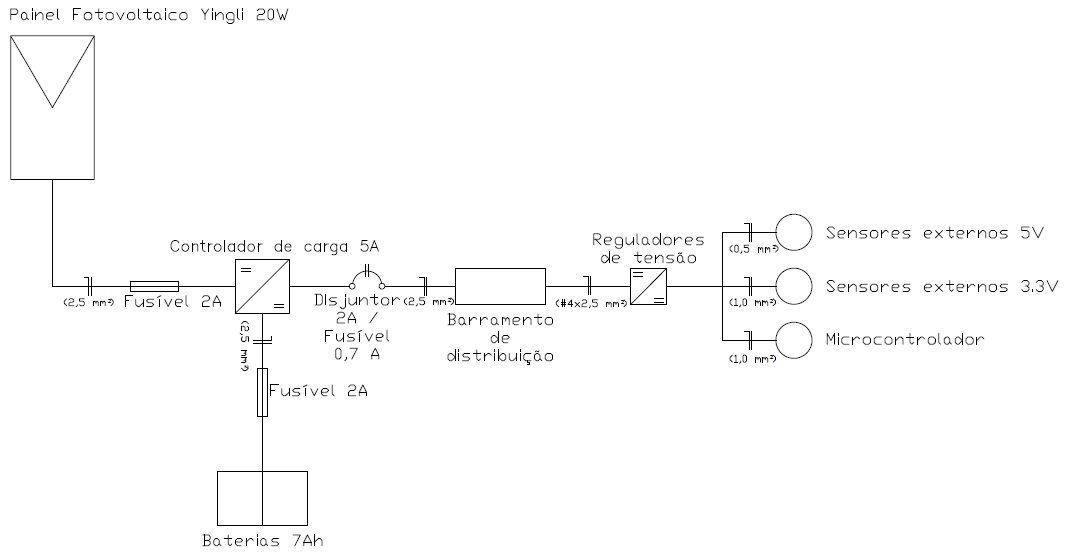
\includegraphics[width = 1 \textwidth]{energia/figuras/ene_pc2_06}
		\caption{Diagrama Unifilar. Fonte:Do Autor}
		\label{ene_pc2_06}
\end{figure}

Este diagrama será a base de contrução de todo o sistema fotovoltaico e todos os demais diagramas apresentados ou utilizados serão derivações ou detalhamentos dele.

\subsection{Simulações}

O PVsyst foi desenvolvido pela Universidade de Genebra (Suíça) e engloba diversos níveis de complexidade permitindo ao usuário trabalhar desde um estágio inicial de representação, com o conceito pré-projeto até um detalhado sistema de simulação de forma completa, podendo este ser simulado para situação de conexão ou não à rede elétrica e também para sistemas fotovoltaicos destinados ao bombeamento de água. Para o projeto condições o software será utilizado para a simulação do sistema fotovoltaico autônomo. \cite{melo}

Para iniciarmos a simulação do sistema, precisamos indicar ao programa a localização onde será instalado o sistema fotovoltaico. Conforme mencionado, o estudo de caso para o projeto considerará uma plantação no DF, portanto o local designado será Brasília-DF. Com a escolha do local também é atrelado a determinação da base de dados de irradiância que para o PVsyst usará, no caso do projeto foi usado o Meteonorm 7.1 para a obtenção dos dados meteorológicos. A figura abaixo mostra os valores de irradiação global obtidos da base de dados adotada pelo PVsyst e vale ressaltar que os valores utilizados são diferentes dos valores utilizados no cálculo teórico já que as bases de dados apresentam resultados ligeiramente diferentes.  

\begin{figure}[H]
		\centering
		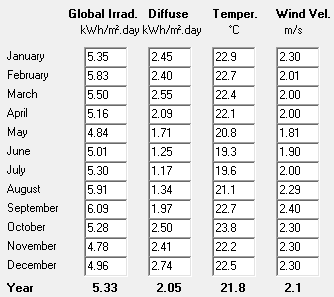
\includegraphics[width = 0.8 \textwidth]{energia/figuras/ene_pc2_dou_01}
		\caption{Valores da radiação solar mensal segundo o PVsyst. Fonte:Do Autor}
		\label{ene_pc2_dou_01}
\end{figure}

Nas configurações para a simulação pode-se alterar os parâmetros Albedo, que é definido como um coeficiente da fração da irradiação incidente global refletida no solo em frente a um plano inclinado. Este efeito acontece durante o cálculo da transposição da irradiação horizontal em um plano inclinado, logo o albedo é nulo no plano horizontal e aumenta conforme a elevação da inclinação. O PVsyst apresenta uma tabela de valores usuais para o albedo.

\begin{table}[]
\caption{Valores usuais para Albedo}
\centering {%
\begin{tabular}{|c|c|}
\hline
\multicolumn{2}{|c|}{Valores usuais para o Albedo} \\ \hline
Ambientes Urbanos & 0,14-0,22 \\ \hline
Grama & 0,15-0,22 \\ \hline
Grama molhada & 0,26 \\ \hline
Neve & 0,82 \\ \hline
Neve derretida & 0,55-0,75 \\ \hline
Asfalto Seco & 0,09-0,15 \\ \hline
Asfalto molhado & 0,18 \\ \hline
Concreto & 0,25-0,35 \\ \hline
Telha cerâmica & 0,33 \\ \hline
Alumínio & 0,85 \\ \hline
Aço Galvanizado Novo & 0,35 \\ \hline
Aço Galvanizado Antigo e sujo & 0,08 \\ \hline
\end{tabular}%
}
\label{ene_pc2_dou_01_tab}
\end{table}

O valor usado será o de 0,20, valor padrão adotado pelo PVsyst. Na prática, exceto para planos verticais, esse valor não assume grande importância pois o componente albedo é relativamente fraco na irradiação global incidente.

No programa foi adicionado a orientação, inclinação e o tipo de estrutura de fixação do módulo fotovoltaico. O módulo fotovoltaico será instalado na estação em um plano inclinado fixo, com uma inclinação de $16\,^{\circ}\mathrm{C}$ e orientado para o norte geográfico. A figura \ref{ene_pc2_dou_02} detalha o que foi citado. 

\begin{figure}[H]
		\centering
		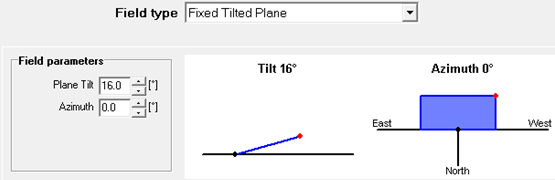
\includegraphics[width = 0.8 \textwidth]{energia/figuras/ene_pc2_dou_02}
		\caption{Inclinação, orientação e tipo de fixação do módulo FV. Fonte:Do Autor}
		\label{ene_pc2_dou_02}
\end{figure}

Com base nesses parâmetros inseridos, o programa nos informa que as perdas devido a orientação ótima são de 0,0 \%, indicando que a orientação e inclinação do módulo está adequada, e o fator de transposição (FT) é de 1,06. Este indicador é definido como a razão entre a irradiação incidente no plano do painel e a irradiação no plano horizontal, mostrando se há ganho ou perda na produção de energia ao inclinar o painel fotovoltaico.

	Ao PVsyst também foi inserido o consumo das cargas diário dos equipamentos presentes na estação, conforme o levantamento de carga feito anteriormente. A Figura \ref{ene_pc2_dou_03} mostra o consumo diário das cargas da estação e o seu consumo mensal.
	
\begin{figure}[H]
		\centering
		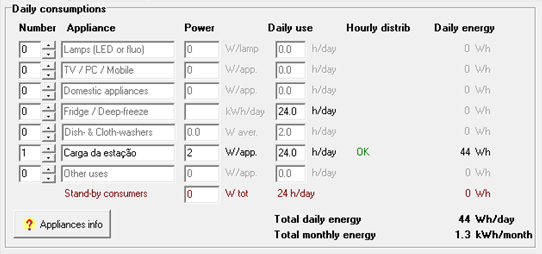
\includegraphics[width = 0.8 \textwidth]{energia/figuras/ene_pc2_dou_03}
		\caption{Consumo diário das cargas da estação inseridos no PVsyst. Fonte:Do Autor}
		\label{ene_pc2_dou_03}
\end{figure}

No PVsyst também foi indicado os componentes do sistema fotovoltaico autônomo, com base no dimensionamento teórico já realizado. O PVsyst possui uma base de dados com vários componentes de sistemas fotovoltaicos, como módulos, controladores, baterias e dentre outros. Esse banco de dados possui um enfoque maior em componentes para sistemas fotovoltaicos \textit{On-grid}, devido ao grande volume de painéis FV de potências nominais elevadas que são direcionados a sistemas conectados a rede. 

Por conta disso, os modelos escolhidos de módulo fotovoltaico, bateria e controlador de carga para o sistema não estão presentes no banco de dados do PVsyst. Logo, para esses três componentes, optou-se em pegar três modelos semelhantes existentes no PVsyst e alterar alguns de seus parâmetros e características nominais, visando torna-los mais próximos dos modelos escolhidos para o projeto. Esses modelos com as características modificadas foram salvos no próprio banco de dados do programa para serem usados na simulação. As figuras a seguir ilustram como os componentes são selecionados no PVsyst.

\begin{figure}[H]
		\centering
		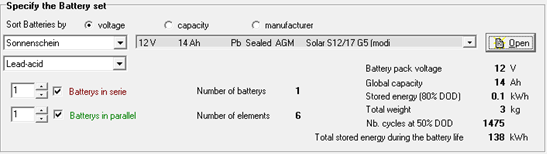
\includegraphics[width = 0.8 \textwidth]{energia/figuras/ene_pc2_dou_04}
		\caption{Selecionando o modelo de bateria no PVsyst. Fonte:Do Autor}
		\label{ene_pc2_dou_04}
\end{figure}

\begin{figure}[H]
		\centering
		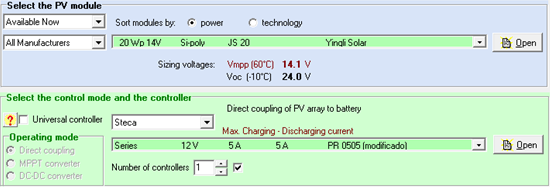
\includegraphics[width = 0.8 \textwidth]{energia/figuras/ene_pc2_dou_05}
		\caption{Selecionando o modelo do módulo fotovoltaico e controlador no PVsyst. Fonte:Do Autor}
		\label{ene_pc2_dou_05}
\end{figure}

Com a determinação dos parâmetros descritos anteriormente, a simulação é executada no PVsyst e os principais resultados são apresentados. A Figura \ref{ene_pc2_dou_06} mostra alguns resultados mensais obtidos da simulação:

\begin{figure}[H]
		\centering
		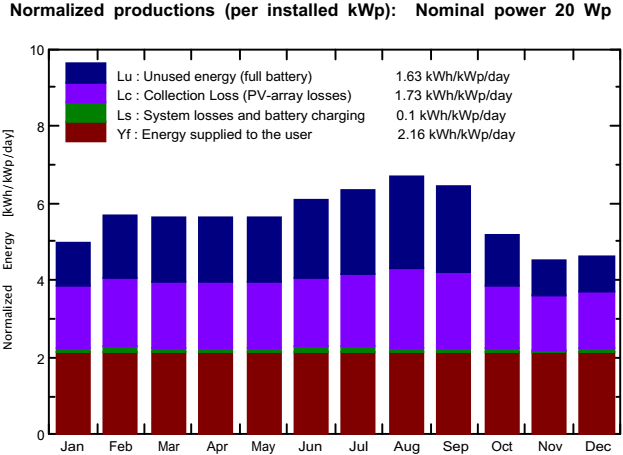
\includegraphics[width = 0.8 \textwidth]{energia/figuras/ene_pc2_dou_06}
		\caption{Produção normalizada pela potência nominal. Fonte:Do Autor}
		\label{ene_pc2_dou_06}
\end{figure}

Onde $Y_f$ é o valor de energia produzido fornecido a carga, cujo o valor médio é de 2,16 $kWh/kWp$ por dia. Já $L_s$ representa as perdas do sistema e de carga da bateria, e seu valor médio diário é de $0,10$ $kWh/kWp$ por dia.  $L_c$ é o valor que descreve as perdas de coleta do módulo, e é a diferença entre a energia incidente no plano do painel e a energia produzida pelo módulo em seus terminais, onde o seu valor médio é de 1,73 $kWh/kWp$ por dia. E a variável $L_u$ corresponde a energia não utilizada, que é a energia produzida e disponível nos terminais do módulo, mas que não pode ser usado por conta de o sistema está saturado, com a bateria carregada. O valor médio de $L_u$ é de $1,63 kWh/kWp$ por dia.

\begin{figure}[H]
		\centering
		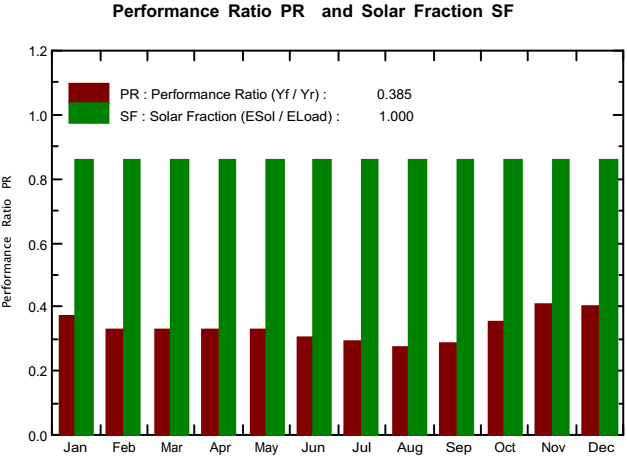
\includegraphics[width = 0.8 \textwidth]{energia/figuras/ene_pc2_dou_07}
		\caption{Taxa de desempenho e fração solar. Fonte:Do Autor}
		\label{ene_pc2_dou_07}
\end{figure}

A fração da energia solar (SF) é a razão entre a energia fornecida a carga pela energia demandada pela carga. O valor médio para a fração solar é 1,0, indicando que o sistema autônomo simulado consegue atender a carga exigida pela estação durante os meses. Além disso o gráfico da figura \ref{ene_pc2_dou_08} mostra a taxa de desempenho (PR) do sistema, que é a eficiência global do sistema em relação a potência nominal instalada e a energia incidente, e apresenta variações durante os meses cujo o valor médio é de 0,385 ou 38,5\%. Idealmente a taxa de desempenho tinha que apresentar um valor médio maior, superior a 0,70, mas devido o valor obtido para a fração solar, as perdas no controlador de carga e as perdas nos reguladores de tensão fazem com que a taxa de desemprenho do sistema seja baixa.

	As informações obtidas das duas últimas figuras podem ser concentradas e resumidas em uma única Tabela \ref{ene_pc2_dou_02_tab}
	
\begin{table}[H]
\caption{Principais resultados da simulação. Fonte do Autor}
\resizebox{\textwidth}{!}{%
\begin{tabular}{|c|c|c|c|c|}
\hline
\multicolumn{5}{|c|}{\textbf{Principais resultados da simulação}} \\ \hline
\multirow{3}{*}{Produção do sistema} & Energia disponível & 28,37 kWh/ano & Produção específica & 1418 kWh/kWp/ano \\ \cline{2-5} 
 & Energia utilizada & 15,77 kWh/ano & Energia não utilizada & 11,89 kWh/ano \\ \cline{2-5} 
 & Taxa de desempenho & 38,49\% & Fração solar (SF) & 100\% \\ \hline
\end{tabular}%
}
\label{ene_pc2_dou_02_tab}
\end{table}

A Tabela \ref{ene_pc2_dou_03_tab} também mostra os balanços e resultados importantes no levantamento de um ano.

\begin{table}[H]
\caption{Balanços e resultados principais. Fonte do Autor}
\resizebox{\textwidth}{!}{%
\begin{tabular}{|c|c|c|c|c|c|c|c|c|}
\hline
 & \textbf{GlobHorkWh/m²} & \textbf{GlobEffkWh/m²} & \textbf{EAvailkWh} & \textbf{EUnusedkWh} & \textbf{EMisskWh} & \textbf{EUserkWh} & \textbf{ELoadkWh} & \textbf{SolFrac} \\ \hline
Jan & 165,8 & 149,2 & 2,114 & 0,709 & 0 & 1,339 & 1,339 & 1 \\ \hline
Fev & 163,3 & 153,5 & 2,179 & 0,884 & 0 & 1,21 & 1,21 & 1 \\ \hline
Mar & 170,4 & 168,7 & 2,409 & 1,01 & 0 & 1,339 & 1,339 & 1 \\ \hline
Abr & 154,8 & 164 & 2,34 & 0,994 & 0 & 1,296 & 1,296 & 1 \\ \hline
Mai & 150 & 169,1 & 2,431 & 1,033 & 0 & 1,339 & 1,339 & 1 \\ \hline
Jun & 150,3 & 177,4 & 2,563 & 1,199 & 0 & 1,296 & 1,296 & 1 \\ \hline
Jul & 164,2 & 191,8 & 2,753 & 1,339 & 0 & 1,339 & 1,339 & 1 \\ \hline
Ago & 183,1 & 202,8 & 2,894 & 1,486 & 0 & 1,339 & 1,339 & 1 \\ \hline
Set & 182,8 & 188,2 & 2,676 & 1,329 & 0 & 1,296 & 1,296 & 1 \\ \hline
Out & 163,7 & 155,6 & 2,207 & 0,817 & 0 & 1,339 & 1,339 & 1 \\ \hline
Nov & 143,5 & 129,9 & 1,847 & 0,531 & 0 & 1,296 & 1,296 & 1 \\ \hline
Dez & 153,8 & 137,2 & 1,957 & 0,563 & 0 & 1,339 & 1,339 & 1 \\ \hline
Ano & 1945,7 & 1987,3 & 28,37 & 11,895 & 0 & 15,768 & 15,768 & 1 \\ \hline
\end{tabular}%
}
\label{ene_pc2_dou_03_tab}
\end{table}
 
	Onde: $Glob_{Hor}$ é a irradiação global no plano horizontal, $Glob_{Eff}$ é a irradiação global efetiva nos coletores depois das perdas ópticas, devido à por exemplo sombreamentos próximos e distantes, a sujeiras no painel, e a efeitos de incidência que causam diminuição da irradiância na cobertura de vidro das células fotovoltaicas; $E_{Avail}$ é a energia solar disponível, que é a energia produzida pelo painel mais a energia não utilizada no sistema; $E_{Unused}$ é a energia não utilizada quando a bateria está cheia;  $E_{Miss}$ é a diferença entre $E_Load$ e $E_{User}$ ($E_{Load}$ – $E_{User}$), sendo $E_{Load}$ a energia requerida pela carga e $E_{User}$ a energia fornecida pelo sistema a carga; e SolFrac a fração solar.
	
	Da tabela anterior podemos observar que a quantidade de energia não utilizada pelo sistema, de cerca de 11,895 kWh, é considerável e se deve a escolha da bateria, pois visando uma economia nos custos optou-se por escolher uma bateria que atende-se bem a demanda da carga, e se negligencio a quantidade de energia que poderia ainda ser aproveitada e armazenada pelo sistema caso fosse escolha uma bateria com uma capacidade de carga maior. 
	
	Da tabela nota-se também que a quantidade anual de energia da irradiação $Glob_{Eff}$ é maior do que a energia da irradiação $Glob_{Hor}$, isso mostra que para o ângulo de inclinação e orientação escolhidos para o módulo, o aproveitamento da irradiação é melhor, pois para determinadas épocas do ano a irradiação global aproveitada no plano inclinado do módulo é maior do que no plano horizontal, no qual não é recomendado a instalação do módulo.

\subsection{Modo de construção}

Está seção destina-se a detalhar algumas partes do processo de contrução do subsistema de alimentação \textit{off-Grid} da estação de medição. O projeto seguirá os esquemáticos e diagramas apresentados na seção de dimencionamento, assim como, os modos de construção citados de modo que está seção apresentá os detalhes finais do processo de construção ainda não abordados no decorrer do capítulo.

\subsubsection{Ocupação dos eletrodutos}

Todo o cabeamento que interconectará os componentes do sistema utilizará os perfis estruturais como eletrodutos. Como os perfis estruturais conectam todas as partes da estrutura e são ocos por dentro (espaço interno de 28,6 x 28,6 mm) foi escolhido passar os fios em seu interior, protegendo o cabeamento e reduzindo os custos com aquisição de eletrodutos. As bordas do furo de entrada e saída dos fios no perfil serão revestidas por polímero de modo a evitar laterais afiadas que possam danificar o isolamento do condutor. Por fim, será utilizado braçadeiras para evitar a movimentação dos cabos dentro dos perfis.

O cabeamento de força sairá em apenas um circuito do quadro e só se ramificará próximo aos sensores que for alimentar de modo a reduzir o número de condutores em cada seção do perfil.

Para confimar que será possível passar todos os condutores com segurança pelo perfil foi calculado a ocupação de cada seção. A figura \ref{ene_pc2_08} apresenta as respectivas seções de eletroduto analisadas e a  tabela \ref{ene_pc2_07_tab} apresenta o número de condutores por trecho do circuito e a ocupação do trecho. 

\begin{figure}[H]
		\centering
		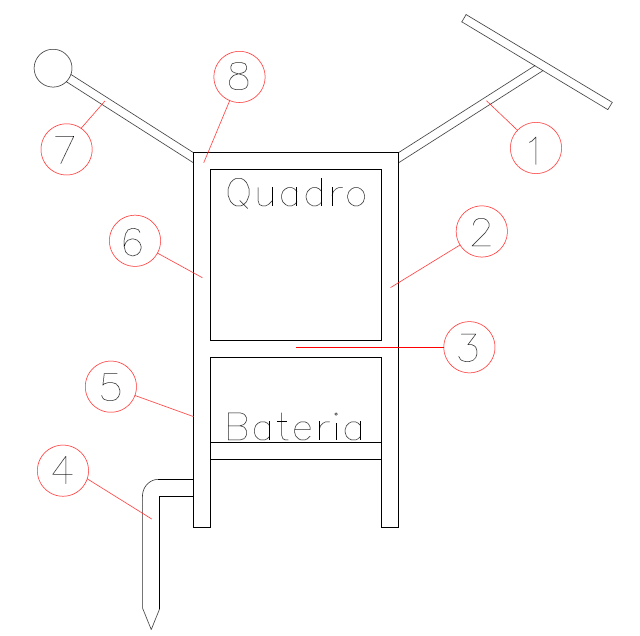
\includegraphics[width = 0.7 \textwidth]{energia/figuras/ene_pc2_08}
		\caption{Esquemático de seções de eletroduto. Fonte:Do Autor}
		\label{ene_pc2_08}
\end{figure}

\begin{table}[]
\caption{Taxa de ocupação das seções do perfil}
\label{ene_pc2_07_tab}
\resizebox{\textwidth}{!}{%
\begin{tabular}{|c|c|c|c|c|c|c|c|c|}
\hline
\textbf{Trecho} & \textbf{Qntd. cabos} & \textbf{Bitola do } & \textbf{Área real do} & \textbf{Qntd. cabos } & \textbf{Bitola do } & \textbf{Área real do } & \textbf{Espaço total} & \textbf{Ocupação} \\ 
&\textbf{de força}&\textbf{condutor ($mm^2$)}&\textbf{condutor ($mm^2$)}&\textbf{de comando}&\textbf{condutor ($mm^2$)}&\textbf{condutor ($mm^2$)}&& \\ \hline
1 & 2 & 2,5 & 9,68 & 0 & 0 & 0 & 23,51 & 2,87\% \\ \hline
2 & 2 & 2,5 & 9,68 & 0 & 0 & 0 & 23,51 & 2,87\% \\ \hline
3 & 4/4/4 & 0,5/1,0/2,5 & 2,19/3,2/9,68 & 20 & 0,14 & 0,4049 & 83,05 & 10,15\% \\ \hline
4 & 6 & 0,5 & 2,19 & 5 & 0,14 & 0,4049 & 18,42 & 14,54\% \\ \hline
5 & 2 & 0,5 & 2,19 & 5 & 0,14 & 0,4049 & 7,78 & 0,95\% \\ \hline
6 & 2/2 & 0,5/1,0 & 2,19/3,2 & 15 & 0,14 & 0,4049 & 21,31 & 2,61\% \\ \hline
7 & 2 & 1,0 & 2,19 & 4 & 0,14 & 0,4049 & 7,26 & 0,89\% \\ \hline
8 & 2/6 & 0,5/1,0 & 2,19/3,2 & 11 & 0,14 & 0,4049 & 28,03 & 3,43\% \\ \hline
\end{tabular}%
}
\end{table}

Segundo a NBR 5410 a ocupação máxima em eletrodutos com três ou mais condutores é de 40\% espaço total do eletroduto. Assim, todos os trechos apresentam ocupação inferior ao limite estabelecido na norma o que confirma que podem ser usados com segurança. 

Para realização dos cálculos foram usados os valores encontrados no catálogo técnico dos fabricantes dos componenetes sendo a Megatron usada para os condutores de força e a marca tiaflex usada para os condutores de comando.

\subsubsection{Emendas de condutores}

Todas as ramificações de circuitos serão realizadas por meio de conectores de emenda tal qual apresentados na figura \ref{ene_pc2_09}. 

\begin{figure}[H]
		\centering
		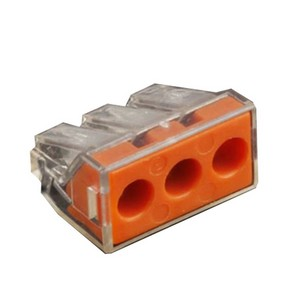
\includegraphics[width = 0.4 \textwidth]{energia/figuras/ene_pc2_09}
		\caption{Conector de emendas}
		\label{ene_pc2_09}
\end{figure}

Os circuitos de força sairão do quadro de distribuição em apenas dois cabos sendo um positivo e um negativo responsável por alimentar as cargas mostradas no diagrama unifilar. Ao chegar próximo aos sensores a serem alimentados as conexões criarão ramificações dos fios que se destinarão a cada sensor específico.

\subsection{Protocolo de Teste}

O processo de testes do subsistema de alimentação \textit{off-Grid} consistirá na medição de seus parâmetros de operação de modo a verificar se o sistema está atendendo aos parâmetros propostos.

Para realização dos testes serão utilizados dois multimetros e uma resistência de 25 $\Omega$ (simula aproximadamente o comportamento dos componentes a serem alimentados) para medir as condições de operação do sistema. Deste modo serão realizados 4 testes.

 \begin{enumerate}
   \item Teste de geração: Será medido a potência gerada pelo painel no decorrer do dia verficando se a geração de energia está acontecendo nos níveis indicados pelo fabricante. Esse teste terá o objetivo de verificar se a geração está acontecendo conforme previsto em projeto.
   \item Teste da bateria: Com a geração desconectada, será medida a potência disponibilizada ao circuito pela bateria de modo a avaliar se o sistema de baterias está funcionando e através do monitoramento da queda de tensão será estimado a autonomia da bateria comparando com o projeto.
   \item Teste de operação continua: O sistema será deixado ao sol por um dia no qual funcionará ininterruptamente de modo que a geração, o nível de bateria e a potência dissipada na resistência de carga possam ser medidas e gerar dados de funcionamento que possam ser comparados com as simulações realizadas para a situação.
   \item Teste dos reguladores de tensão: Será medida a tensão e a corrente na entrada e na saída do regulador de tensão de modo a verificar se a tensão está no nível certo de alimentação e para medir a eficiência real no caso do projeto para este componente.
 \end{enumerate}

\section{Atuador}

Um dos requisitos do projeto é realizar o acionamento do sistema de irrigação de forma automática caso o usuário decida por este modo. Assim, foi necessário projetar um módulo de acionamento remoto que atue no quadro de comando do sistema de irrigação e esteja em paralelo com o sistema atual de acionamento. 

Foi analisada a viabilidade de realizar o acionamento das bombas através de um módulo comercial de acionamento remoto. Porém estes equipamentos possuem valores acima do orçamento de projeto, além de utilizarem módulos e protocolos prontos de comunicação dificultando a integração com o resto do sistema. Além do fato de que funcionam como uma caixa preta recebendo um input e tendo como saída um output fixo, de modo que não se entende bem como ocorre seu funcionamento interno.

Assim, optou-se pela construção de um módulo de acionamento próprio que ficasse localizado próximo ao quadro de acionamento da irrigação e fizesse parte da rede mesh, acionando ou desligando a irrigação conforme a necessidade.

\subsection{Esquemático do módulo}

O atuador será construído dentro de um quadro de comando tal qual o utilizado no projeto da estação. Será utilizado o nível de proteção IP65 nele, pois o sistema pode ser acoplado a diversos tipo de fazenda, logo é preciso garantir que os componentes internos estejam protegidos independente da estrutura física de onde seja instalado.

Assim, o sistema do atuador seguirá o esquemático apresentado na figura \ref{ene_pc2_07}.

\begin{figure}[H]
		\centering
		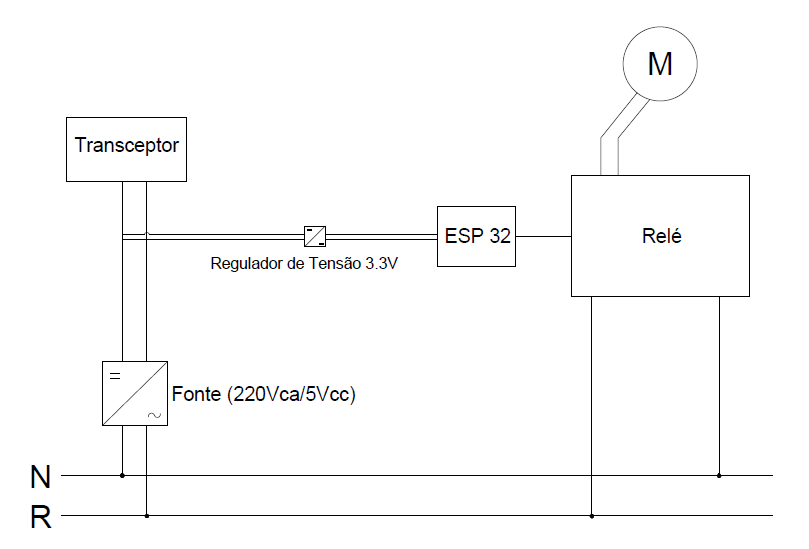
\includegraphics[width = 0.9 \textwidth]{energia/figuras/ene_pc2_07}
		\caption{Esquemático do atuador. Fonte:Do Autor}
		\label{ene_pc2_07}
\end{figure}

A fonte apresentada no esquemático será projeta e construída pela divisão de energia do projeto e deverá realizar o abaixamento da tensão de 220 V para 5 V, além de retificar o sinal convertendo-o de corrente alternada para corrente contínua. Outros fatores como ripple de funcionamento e parâmetros de projeto serão apresentados na seção seguinte.

O transceptor e o microcontrolador utilizado serão iguais aos presentes na estação de modo a atender os requisitos expostos na seção de eletrônica. 

Além disso, o regulador de tensão utilizado será o módulo regulador buck LM2596 e será responsável por abaixar a tensão de 5 V da fonte para 3,3 V de modo a alimentar o microcontrolador. Assim, haverá uma padronização dos equipamentos utilizados na estação e no atuador facilitando a aquisição de materiais e posteriormente o escalonamento da produção.

Ainda, o microcontrolador realiza o acionamento do módulo relé ligando ou desligando a irrigação conforme o necessário. Como exposto no ponto de controle 1, o sistema deve ser alterado de acordo com as características do sistema de irrigação que se deseja partir ajustando os componentes para suportar as correntes e regimes de operação específicos da aplicação. 

No caso do projeto, será utilizada uma bomba bomba de poço artesiano modelo 1650 da HS para simular o sistema de irrigação, tal bomba não faz parte do projeto em si, mas será usada para demonstrar o funcionamento do sistema de acionamento a distância. Está bomba apresenta potência de 320 W e corrente nominal de 1,45 A.

Assim, o módulo relé a ser utilizado será de 220V e 10 A com alimentação de 3,3 Vcc. Este modelo apresenta uma corrente de operação superior a corrente nominal da bomba, porém é o equipamento comercial que melhor atende ao projeto e que pode ser comandado pelo microcontrolador de modo que será utilizado e promoverá o aumento da robustez do sistema.

Por fim, foi construído o diagrama unifilar do sistema de modo a guiar a construção. A figura \ref{ene_pc2_13} apresenta o diagrama traçado e a tabela \ref{ene_pc2_10_tab} apresenta as grandezas utilizadas para o dimensionamento dos condutores.

\begin{figure}[H]
		\centering
		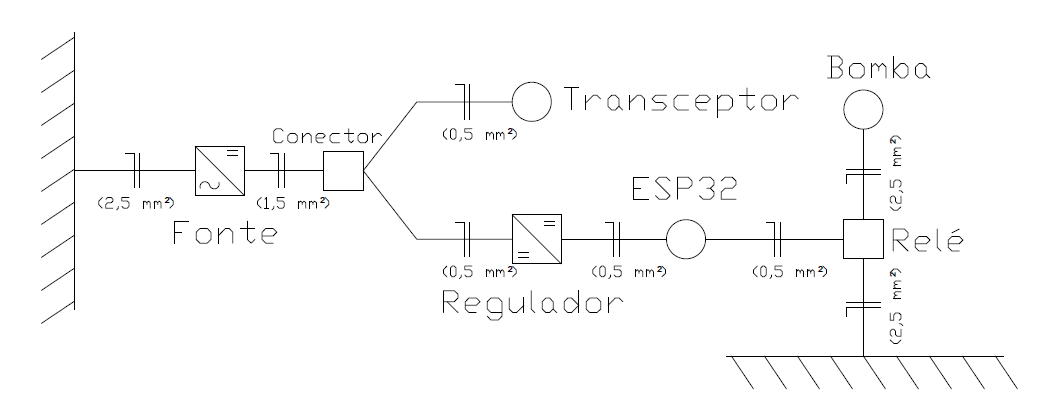
\includegraphics[width = 0.9 \textwidth]{energia/figuras/ene_pc2_13}
		\caption{Diagrama unifilar do atuador. Fonte:Do Autor}
		\label{ene_pc2_13}
\end{figure}

\begin{table}[H]
\caption{Dimensionamento dos condutores de força do atuador}
\resizebox{\textwidth}{!}{%
\begin{tabular}{|c|c|c|c|c|c|c|}
\hline
\textbf{Cabeamentos} & \textbf{Distância} & \textbf{Corrente} & \textbf{Queda de tensão planejada} & \textbf{Bitola do condutor} & \textbf{Bitola comercial (mm²)} & \textbf{Queda de tensão real} \\ \hline
rede/fonte & 1,5 & 0,35 & 1,00\% & 0,932 & 2,5 & 0,37\% \\ \hline
fonte/conector & 0,1 & 0,35 & 0,50\% & 0,124 & 1,5 & 0,04\% \\ \hline
conector-transceptor & 0,1 & 0,02 & 0,50\% & 0,006 & 0,5 & 0,01\% \\ \hline
conector-regulador & 0,1 & 0,33 & 0,15\% & 0,395 & 0,5 & 0,12\% \\ \hline
regulador-esp & 0,1 & 0,33 & 0,15\% & 0,388 & 0,5 & 0,12\% \\ \hline
esp-relé & 0,1 & 0,03 & 0,15\% & 0,030 & 0,5 & 0,01\% \\ \hline
rede-relé & 2 & 1,82 & 4,00\% & 1,627 & 2,5 & 2,604\% \\ \hline
relé-bomba & 2 & 1,82 & 4,00\% & 1,627 & 2,5 & 2,60\% \\ \hline
\end{tabular}%
}
\label{ene_pc2_10_tab}
\end{table}

\subsection{Dimensionamento da fonte}



\subsection{Modo de construção}

Será utilizado o mesmo modelo de quadro usado na estação para construção do módulo atuador. O quadro será responsável por abrigar todos os componentes e protegê-los de intempéries e outros dados que podem vir a sofrer. O esquemático abaixo apresenta a disposição dos componenetes na estrutura:

\begin{figure}[H]
		\centering
		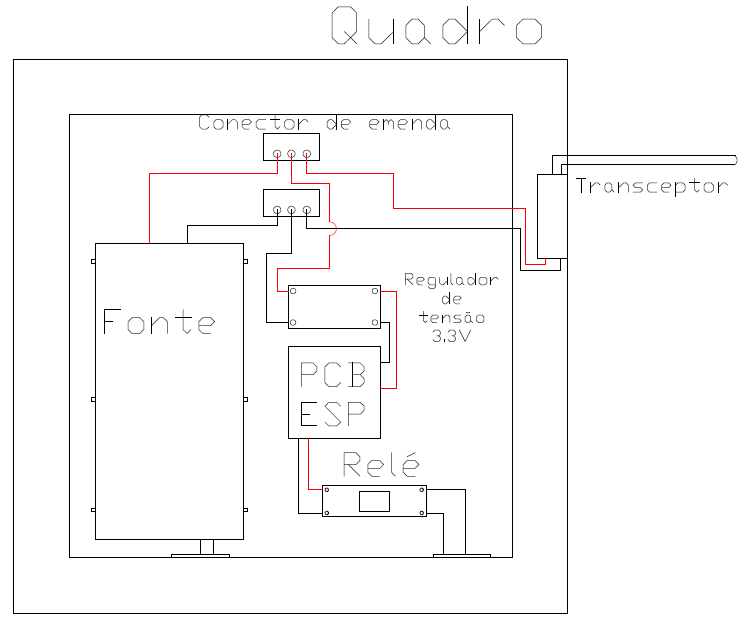
\includegraphics[width = 0.9 \textwidth]{energia/figuras/ene_pc2_10}
		\caption{Posicionamento dos componentes no quadro do atuador. Fonte:Do Autor}
		\label{ene_pc2_10}
\end{figure}

Para a fixação da fonte, da PCE e do módulo regulador de tensão serão utilizados parafusos Inox 304 (A2) com ranhura phillips e dimensões M2 e 5 mm de comprimento. Está opção foi escolhida, pois os componentes já apresentam locais específicos para serem fixados.

Já os conectores de emenda e o transceptor serão fixados ao quadro por meio de braçadeiras de fixação.

Por fim, a antena do transceptor precisará ficar do lado de fora do quadro, de modo que será realizado a vedação em torno de seu furo de modo a evitar a entrada de água no quadro.

\subsection{Protocolo de testes}

Os testes do atuador serão realizados em parceria com a área de sistemas eletrônicos e visarão demonstrar que o módulo opera conforme o projetado. Para isso, serão usados um osciloscópio e uma lâmpada de Led para realizar os testes.

\begin{enumerate}
   \item Teste da fonte: Antes de conectar os demais compoenetes ao circuito, será testado se a fonte contruída pelo grupo realmente atende aos parâmetros estipulados em seu projeto. Assim, será utilizado o osciloscópio para medir a saída da fonte e calcular os parâmetros de interesse. 
   \item Teste de acionamento: A lâmpada de led será ligada na saída do módulo relé como sendo a carga do sistema. Será enviado um sinal para o transceptor do atuador de modo a abrir o relé e ascender a lâmpada demonstrando o conceito por trás do acionamento do sistema de irrigação a distância.
    \end{enumerate}

\section{Central}

A central de comando será responsável por comunicar as informações medidas nas estações com a aplicação web de modo que será o único ponto do sistema com acesso obrigatório a internet. 

\subsection{Esquemático da central}

Do ponto de vista da alimentação elétrica, a central será alimentada por uma fonte semelhante a dimensionada no capítulo do atuador seguindo o diagrama unifilar apresentado a baixo:

\begin{figure}[H]
		\centering
		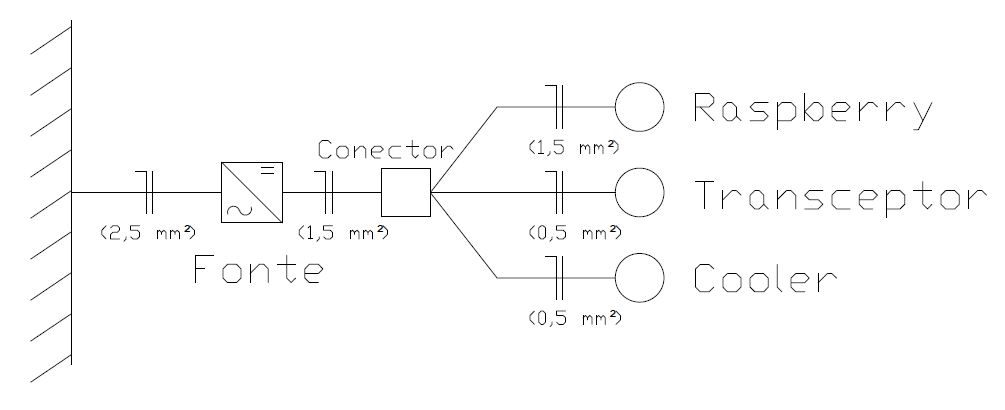
\includegraphics[width = 0.9 \textwidth]{energia/figuras/ene_pc2_12}
		\caption{Diagrama unifilar da central de comando. Fonte:Do Autor}
		\label{ene_pc2_12}
\end{figure}

A metodologia para dimensionar os condutores do sistema foi realizada da mesma maneira apresentada na seção de dimensionamento do cabeamento da instalação. Assim, a tabela \ref{ene_pc2_09_tab} apresenta as grandezas utilizadas no dimensionamento.

\begin{table}[H]
\caption{Dimensionamento do cabeamento de força da central.}
\resizebox{\textwidth}{!}{%
\begin{tabular}{|c|c|c|c|c|c|c|}
\hline
\textbf{Cabeamentos} & \textbf{Distância} & \textbf{Corrente} & \textbf{Queda de tensão planejada} & \textbf{Bitola do condutor} & \textbf{Bitola comercial (mm²)} & \textbf{Queda de tensão real} \\ \hline
Rede-Fonte & 1,5 & 3,39 & 4\% & 2,274 & 2,5 & 3,64\% \\ \hline
Fonte-conector & 0,1 & 3,39 & 0,50\% & 1,213 & 1,5 & 0,40\% \\ \hline
conector-raspberry & 0,1 & 3,13 & 0,50\% & 1,119 & 1,5 & 0,37\% \\ \hline
conector-transceptor & 0,1 & 0,02 & 0,50\% & 0,006 & 0,5 & 0,01\% \\ \hline
conector-cooler & 0,1 & 0,25 & 0,50\% & 0,090 & 0,5 & 0,090\% \\ \hline
\end{tabular}%
}
\label{ene_pc2_09_tab}
\end{table}

\subsection{Modo de construção}

Para a central, será utilizado um quadro de comando de 30x20x20 cm com placa de montagem interna de modo a facilitar a organização dos componentes. O esquemático a seguir apresenta o posicionamentos dos componentes dentro do quadro.

\begin{figure}[H]
		\centering
		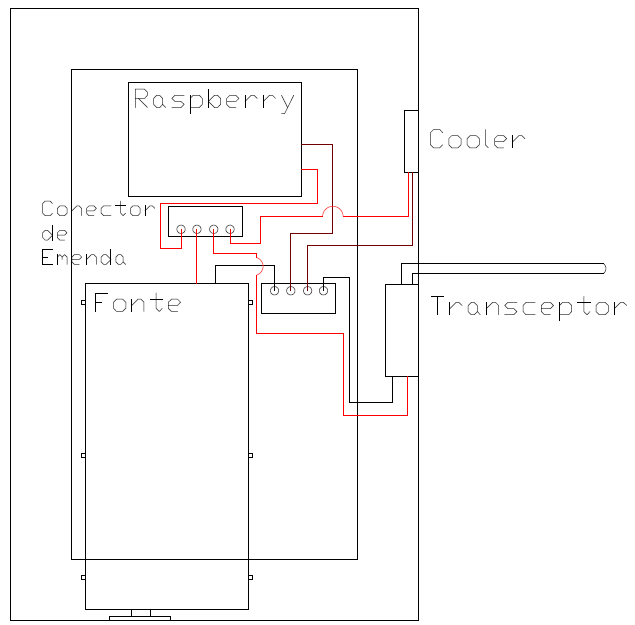
\includegraphics[width = 0.9 \textwidth]{energia/figuras/ene_pc2_11}
		\caption{Posicionamento dos componentes no quadro da central. Fonte:Do Autor}
		\label{ene_pc2_11}
\end{figure}

Os componentes serão fixados na placa de montagem através de parafusos Inox 304 (A2) com ranhura pphillips e dimensões M2 e 5 mm quando o componente possuir suporte individual. (fonte, raspberry e cooler). Os demais componentes serão fixados no quadro através de braçadeiras de fixação.

\subsection{Protocolo de teste}

Para testar o funcionamento da parte elétrica da central de comando, será usado um osciloscópio. O teste visará medir os parâmetros elétricos na saída da fonte e nos pontos de alimentação de cada componente de modo a analisar se a fonte cumpre seus parâmetros de projeto e se os componentes estão sendo alimentados de forma apropriada.